\documentclass[xcolor=pdftex,romanian,colorlinks]{beamer}
%\documentclass[xcolor=pdftex,handout,romanian,colorlinks]{beamer}

\usepackage[export]{adjustbox}
\usepackage{../sty/tslides}
\usepackage[all]{xy}
\usepackage{pgfplots}
\usepackage{flowchart}
\usepackage{todonotes}
\usetikzlibrary{arrows,positioning,calc}
\lstset{language=Haskell}
\lstset{escapeinside={(*@}{@*)}}
\PrerenderUnicode{ăĂîÎȘșȚțâÂ}

%\usepackage{xcolor}
%\definecolor{IntensColor}{HTML}{2E86C1}
%\definecolor{StateTransition}{HTML}{D6EAF8}
%\definecolor{MedianLightOrange}{RGB}{216,178,92}
%\definecolor{Orchid}{HTML}{8E44AD}
%\definecolor{True}{HTML}{229954}
%\definecolor{False}{HTML}{CB4335}


\usepackage{proof}
\usepackage{multirow}
\usepackage{alltt}
\usepackage{mathpartir}
\usepackage{ulem}

\newcommand{\structured}[1]{#1}

\definecolor{IntensColor}{HTML}{2E86C1}
\definecolor{StateTransition}{HTML}{D6EAF8}
\definecolor{MedianLightOrange}{RGB}{216,178,92}
\definecolor{Orchid}{HTML}{8E44AD}
\definecolor{True}{HTML}{229954}
\definecolor{False}{HTML}{CB4335}

\newcommand{\cin}[1]{{\color{cobalt} #1}}
\newcommand{\sel}[1]{{\color{Orchid} #1}}

\newcommand{\intens}[1] {{\color{IntensColor} #1}}
\newcommand{\exe}[1] {{\color{True} #1}}

\newcommand{\la}{\lambda}

\setlength{\leftmargini}{0pt}

\newcommand{\app}[2]{#1\, #2}
\newcommand{\abs}[2]{\lambda #1.\,#2}

\newcommand{\type}[2]{{\color{True}#1\hspace{-.05cm}:}\,{\color{Orchid}#2}}

\newcommand{\sub}[3]{#1\langle#2/#3\rangle}
\newcommand{\subt}[3]{#1[#2/#3]}
\newcommand{\equiva}{=_\alpha}

\newcommand{\trueL}{\mathbf{T}}
\newcommand{\falseL}{\mathbf{F}}
\newcommand{\notL}{\mathbf{not}}
\newcommand{\andL}{\mathbf{and}}
\newcommand{\orL}{\mathbf{or}}
\newcommand{\ifL}{\mathbf{if}}
\newcommand{\boolL}{\mathbf{bool}}

\newcommand{\maybeL}{\mathbf{maybe}}
\newcommand{\nothingL}{\mathbf{Nothing}}
\newcommand{\justL}{\mathbf{Just}}
\newcommand{\Maybe}[1]{\mathop{\mathbf{Maybe}}{#1}}

\newcommand{\foldrL}{\mathbf{foldr}}
\newcommand{\nilL}{\mathbf{Nil}}
\newcommand{\consL}{\mathbf{Cons}}
\newcommand{\ListL}[1]{\mathop{\mathbf{List}}{#1}}

\newcommand{\unpairL}{\mathbf{uncons}}
\newcommand{\pairL}{\mathbf{Pair}}
\newcommand{\firstL}{\mathbf{first}}
\newcommand{\secondL}{\mathbf{second}}
\newcommand{\Pair}[2]{\mathop{\mathop{\mathbf{Pair}}{#1}}{#2}}

\newcommand{\succL}{\mathbf{Succ}}
\newcommand{\zeroL}{\mathbf{Zero}}
\newcommand{\iterateL}{\mathbf{iterate}}
\newcommand{\addL}{\mathbf{add}}
\newcommand{\mulL}{\mathbf{mul}}
\newcommand{\expL}{\mathbf{exp}}
\newcommand{\isZero}{\mathbf{isZero}}
\newcommand{\pred}{\mathbf{pred}}
\newcommand{\factL}{\mathbf{fact}}

\newcommand{\BoolT}{\ensuremath{\texttt{Bool}}}
%\newcommand{\BoolT}{\ensuremath{\texttt{Bool}}}
\newcommand{\ifT}[3]{\mathrm{if}\ #1\ \mathrm{then}\ #2\ \mathrm{else}\ #3}

\newcommand{\UnitT}{\ensuremath{\texttt{Unit}}}
\newcommand{\unit}{\mathrm{unit}}

\newcommand{\VoidT}{\ensuremath{\texttt{Void}}}
\newcommand{\void}{\mathrm{void}}


\newcommand{\ProductT}[2]{#1 \times #2}
\newcommand{\PairL}[2]{\langle #1,#2\rangle}
\newcommand{\ProjOne}[1]{fst\ #1}
\newcommand{\ProjTwo}[1]{snd\ #1}

\newcommand{\SumT}[2]{#1 + #2}
\newcommand{\Left}[1]{\mathrm{Left}\ #1}
\newcommand{\Right}[1]{\mathrm{Right}\ #1}
\newcommand{\Case}[3]{\mathrm{case}\ #1\ \mathrm{of}\ #2\ ;\ #3}

%----------------------------------------------

\newcommand{\SSnot}{\terminal{not}}

\newcommand{\Sand}{\terminal{and}}
\newcommand{\Sor}{\terminal{or}}
\newcommand{\Splus}{\terminal{+}}
\newcommand{\Smul}{\terminal{*}}
\newcommand{\Ssucc}{\terminal{S}}
\newcommand{\Spow}{\terminal{pow}}
\newcommand{\Spred}{\terminal{pred}}
\newcommand{\Seq}{\terminal{eq}}
\newcommand{\Sneq}{\terminal{neq}}

\newcommand{\SisZero}{\terminal{isZero}}
\newcommand{\Slte}{\terminal{<=}}
\newcommand{\Sgte}{\terminal{>=}}
\newcommand{\Slt}{\terminal{<}}
\newcommand{\Sgt}{\terminal{>}}
\newcommand{\Spair}{\terminal{pair}}
\newcommand{\Sfst}{\terminal{fst}}
\newcommand{\Ssnd}{\terminal{snd}}
\newcommand{\Sminus}{\terminal{-}}

\newcommand{\Snull}{\terminal{null}}
\newcommand{\Scons}{\terminal{cons}}
%\newcommand{\c sead}{\terminal{head}}
\newcommand{\SisNull}{\terminal{?null}}
\newcommand{\Stail}{\terminal{tail}}
\newcommand{\Ssum}{\terminal{sum}}
\newcommand{\Sfoldr}{\terminal{foldr}}
\newcommand{\Smap}{\terminal{map}}
\newcommand{\Sfilter}{\terminal{filter}}

\newcommand{\const}[1]{\triangleright {\color{False} #1}}

\newcommand{\egf}[1]{\stackrel{\cdot}{=}_{#1}}

\newcommand{\Conf}[2]{\ensuremath{\langle #1\ ,\ #2\rangle}}
\newcommand{\plus}[1] {{\color{True} #1}}
\newcommand{\te}[1]{\mbox{\texttt{#1}}}

\newcommand{\vexp}{\ensuremath{\mathbb{E}}}
\newcommand{\bexp}{\ensuremath{\mathbb{B}}}
\newcommand{\cmd}{\ensuremath{\mathbb{C}}}

\definecolor{section-color}{HTML}{23373b} %mDarkTeal
%\AtBeginSection[]{
%  \begin{frame}
%  \vfill
%  \centering
%  \begin{beamercolorbox}[sep=8pt,center,shadow=true,rounded=true]{title}
%    \usebeamerfont{title}\insertsectionhead\par%
%  \end{beamercolorbox}
%  \vfill
%  \end{frame}
%}



\title[FLP]{Fundamentele limbajelor de programare}
\subtitle{C02}
\date{}


\begin{document}
\begin{frame}
  \titlepage
\end{frame}

%================================================
\section{\color{section-color} Lambda calcul - elemente de bază}
%================================================

\begin{frame}{Lambda calcul}

\begin{itemize}
	\medskip
	\item Un model de calculabilitate
	\medskip
	\item Limbajele de programare funcțională sunt extensii ale sale
	\medskip
	\item Un limbaj formal
	\medskip
	\item Expresiile din acest limbaj se numesc \alert{lambda termeni}
	\medskip
	\item Vom defini reguli pentru a îi manipula
\end{itemize}
\end{frame}

%------------------------------------------------
\begin{frame}{Lambda termeni}

Fie $V$ o mulțime infinită de variabile, notate $x,y,z,\dots$. 

Mulțimea \intens{lambda termenilor} este dată de următoarea formă BNF:
\vspace{-.4cm}
\begin{center}
\begin{tabular}{rcl}
\intens{lambda termen} & =  &  \intens{variabilă}\\
& | & \intens{aplicare} \\
& | & \intens{abstractizare}
\end{tabular}

\alert{$M,N ::= x\ |\ (\app{M}{N})\ |\ (\abs{x}{M})$}
\end{center}


\begin{example}
\begin{columns}
\begin{column}{.4\textwidth}
\begin{itemize}
	\item $x, y, z$
	\item $(\app{x}{y}), (\app{y}{x})$, $(\app{x}{(\app{yx})})$
	\item $(\abs{x}{x}), \abs{x}{(\app{x}{y})}, \abs{z}{(\app{x}{y})}$

\end{itemize}
\end{column}
\begin{column}{.4\textwidth}
\begin{itemize}
	\item $(\app{(\abs{x}{x})}{y}), (\app{(\abs{x}{(\app{x}{z})})}{y})$
	\item $(\abs{f}{(\abs{x}{(\app{f}{(\app{f}{x})})})})$
	\item $\app{(\abs{x}{x})}{(\abs{x}{x})}$
\end{itemize}
\end{column}
\end{columns}
\end{example}
\end{frame}

%------------------------------------------------
\begin{frame}[fragile]{Funcții anonime în Haskell}

\begin{center}
\begin{tabular}{rcl}
\intens{lambda termen} & =  &  \intens{variabilă}\\
& | & \intens{aplicare} \\
& | & \intens{abstractizare}
\end{tabular}

\alert{$M,N ::= x\ |\ (\app{M}{N})\ |\ (\abs{x}{M})$}
\end{center}


 În Haskell, \structure{\textbackslash} e folosit în locul simbolului \structure{$\lambda$} și
 \structure{\lstinline{->}} în locul punctului:

\begin{tabular}{c@{ este  }c}
$\lambda x. x * x$ & \texttt{\textbackslash x -> x * x}
\\
$\lambda x. x > 0$ & \texttt{\textbackslash x -> x > 0}
\end{tabular}

\end{frame}

%------------------------------------------------
\begin{frame}{Lambda termeni - definiție alternativă}

Fie $V$ o mulțime infinită de variabile, notate $x,y,z,\dots$. 

Fie $A$ un alfabet format din elementele din $V$, și simbolurile speciale $"("$, $")"$, $"\la"$ si $"."$

Fie $A^*$ mulțimea tuturor cuvintelor finite pentru alfabetul $A$. 

\bigskip
Mulțimea \intens{lambda termenilor} este cea mai mică submulțime $\intens{\Lambda} \subseteq A^*$ astfel încât:
\vspace{-.2cm}
\begin{itemize}
\item[][\intens{Variabilă}] \alert{$V \subseteq \Lambda$}
\item[][\intens{Aplicare}] dacă $M,N \in \Lambda$ atunci 
\alert{$(M\, N)\in \Lambda$}
\item[][\intens{Abstractizare}] dacă $x\in V$ și $M\in \Lambda$ atunci \alert{$(\la x.M)\in \Lambda$}
\end{itemize} 
\end{frame}


%------------------------------------------------
\begin{frame}[fragile]{ Convenții}

\begin{itemize}
\item Se elimină parantezele exterioare
\medskip
\item Aplicarea este asociativă la stânga \\
\begin{itemize}
	\item \intens{$\app{\app{M}{N}}{P}$} înseamnă \intens{$\app{(\app{M}{N})}{P}$}\\
	\item \intens{$\app{\app{\app{f}{x}}{y}}{z}$} înseamnă \intens{$\app{(\app{(\app{f}{x})}{y})}{z}$} 
\end{itemize}

\medskip
\item Corpul abstractizării (partea de după punct) se extinde la dreapta cât se poate
\begin{itemize}
	\item \intens{$\abs{x}{\app{M}{N}}$} înseamnă \intens{$\abs{x}{(\app{M}{N})}$}, nu {\color{red} $\app{(\abs{x}{M})}{N}$}
\end{itemize}

\medskip
\item Mai mulți $\lambda$ pot fi comprimați
\begin{itemize}
	\item \intens{$\abs{xyz}{M}$} este o abreviere pentru \intens{$\abs{x}{\abs{y}{\abs{z}{M}}}$}
\end{itemize}
\end{itemize}

Aceste convenții nu afectează definiția lambda termenilor.
\end{frame}

\setlength{\leftmargini}{15pt}

%------------------------------------------------
\begin{frame}[fragile]{Exerciții}

\textbf{\intens{Exercițiu.}} 
Scrieți termenii de mai jos cu cât mai puține paranteze și folosind convențiile de mai sus, fără a schimba sensul  termenilor:
\begin{enumerate}
	\item \alert{$(\abs{x}{(\abs{y}{(\abs{z}{((\app{x}{z})(\app{y}{z}))})})})$} 
	\onslide<2->{\hfill {\color{True} Corect:  $\abs{xyz}{\app{\app{x}{z}}(\app{y}{z})}$}}
	
	\smallskip
	\item \alert{$(\app{(\app{(\app{a}{b})}{(\app{c}{d})})}{(\app{(\app{e}{f})}{(\app{g}{h})})})$} 
	\onslide<3->{\hfill {\color{True} Corect:  $\app{\app{\app{a}{b}}{(\app{c}{d})}}{(\app{\app{e}{f}}{(\app{g}{h})})}$}}
	
%	\medskip
%	\item \alert{$\app{(\abs{x}{\app{\app{(\app{\app{(\abs{y}{(\app{y}{x})})}}{(\abs{v}{v})}}{z})}}{u}}){(\abs{w}{w})}$} \\
%	\onslide<4->{$\app{(\abs{x}{\app{\app{(\app{\app{(\abs{y}{(\app{y}{x})})}}{(\abs{v}{v})}}{z})}}{u}}){(\abs{w}{w})}$}
\end{enumerate}

\bigskip
\textbf{\intens{Exercițiu.}} Adăugați parantezele în termenii de mai jos astfel încât să nu le schimbați sensul:
\begin{enumerate}
	\item \alert{$\app{\app{\app{x}{x}}{x}}{x}$} 
	 \onslide<4->{\hfill {\color{True} Corect: $(\app{(\app{(\app{x}{x})}{x})}{x})$}}
	 
	 \smallskip
	 \item \alert{$\abs{x}{\app{x}{\abs{y}{y}}}$}
	 \onslide<5->{\hfill {\color{True} Corect:  $(\abs{x}{(\app{x}{(\abs{y}{y})})})$}}
\end{enumerate} 
\end{frame}
%------------------------------------------------

\begin{frame}[fragile]{ Variabile libere și variabile legate}

\begin{itemize}
\item $\abs{\_}{\_}$ se numește operator \alert{de legare} (\textit{binder})
\item $x$ din $\abs{x}{\_}$ se numește variabilă \alert{de legare} (\textit{binding})
\item $N$ din $\abs{x}{N}$ se numește \alert{domeniul} (\textit{scope}) de legare a lui $x$
\item toate aparițiile lui $x$ în $N$ sunt legate
\item O apariție care nu este legată se numește \alert{liberă}.
\item Un termen fără variable libere se numește \alert{închis} (\textit{closed}). 
\item Un termen închis se mai numește și \alert{combinator}.
\end{itemize}

\bigskip
De exemplu, în termenul
\vspace{-.4cm}
\begin{center}
\intens{$M \equiv \app{(\abs{x}{xy})}{(\abs{y}{yz})}$}
\end{center}
\vspace{-.6cm}
\begin{itemize}
	\item $x$ este legată
	\item $z$ este liberă
	\item $y$ are și o apariție legată, și una liberă
	\item mulțimea variabilelor libere ale lui $M$ este $\{y,z\}$
\end{itemize}
\end{frame}

%------------------------------------------------

\begin{frame}[fragile]{ Variabile libere}


Mulțimea \alert{variabilelor libere} dintr-un termen $M$ este notată $FV(M)$ și este definită formal prin:
\begin{center}
\begin{tabular}{rcl}
$FV(x)$ & $=$ & $\{x\}$ \\
$FV(\app{M}{N})$ & $=$ & $FV(M) \cup FV(N)$ \\
$FV(\abs{x}{M})$ & $=$ & $FV(M) \setminus \{x\}$ \\
\end{tabular}
\end{center}

Exemplu de definiție recursivă pe termeni. Adică în definiția lui $FV(M)$ am presupus că am definit deja $FV(N)$ pentru toți subtermenii lui $M$.

\begin{example}
\begin{itemize}
\item $FV(\abs{x}{\app{x}{y}}) = FV(\app{x}{y}) \setminus \{x\} = (FV(x)\cup FV(y))\setminus \{x\} $ \\
	\hspace{1.8cm} $ = (\{x\}\cup \{y\}) \setminus \{x\} = \{y\}$
\item $FV(\app{x}{\abs{x}{\app{x}{y}}}) = \{x, y\}$
\end{itemize}
\end{example}
\end{frame}

%------------------------------------------------

\begin{frame}[fragile]{Redenumire de variabile}

\intens{Ce înseamnă să redenumim o variabilă într-un termen?}

\smallskip
Dacă $x,y$ sunt variabile și $M$ este un termen, \intens{$\sub{M}{y}{x}$} este rezultatul obținut după redenumirea lui $x$ cu $y$ în $M$. 

\vspace{-.8cm}
\begin{center}
\begin{flalign*}
\sub{x}{y}{x} & \equiv  y,  \\
\sub{z}{y}{x} & \equiv  z, \hspace{2.4cm} \mbox{dacă } x \neq z\\
\sub{(\app{M}{N})}{y}{x} & \equiv \app{(\sub{M}{y}{x})}{(\sub{N}{y}{x})} \\
\sub{(\abs{x}{M})}{y}{x} & \equiv \abs{y}{(\sub{M}{y}{x})} \\
\sub{(\abs{z}{M})}{y}{x} & \equiv \abs{z}{(\sub{M}{y}{x})}, \hspace{.6cm} \mbox{dacă } x \neq z\\
\end{flalign*}
\end{center}

\vspace{-.7cm}
Observați că acest tip  de redenumire înlocuiește toate aparițiile lui $x$ cu $y$, indiferent dacă este liberă, legată, sau de legare.

Se folosește doar în cazuri în care $y$ nu apare deja în $M$.
\end{frame}

%------------------------------------------------

\begin{frame}[fragile]{$\alpha$-echivalență}

\intens{Ce înseamnă că doi termeni sunt egali,}\\ 
\intens{\textbf{modulo redenumire de variabile legate}?}

\smallskip
Definim \alert{$\alpha$-echivalența} ca fiind cea mai mică relație de congruență $\equiva$ pe mulțimea lambda termenilor, astfel încât pentru orice termen $M$ și orice variabilă $y$ care nu apare în $M$, avem
\vspace{-0.4cm}
\begin{center}
\intens{$\abs{x}{M}\ \equiva\ \abs{y}{(\sub{M}{y}{x})}$}
\end{center} 

%Doi termeni sunt $\alpha$-echivalenți dacă au toate variabilele legate distincte între ele și de orice variabilă liberă.
\end{frame}

%------------------------------------------------

\begin{frame}[fragile]{$\alpha$-echivalență}

$\alpha$-echivalența \intens{$=_\alpha$} este cea mai mică relație pe lambda termeni care satisface regulile:

\begin{center}
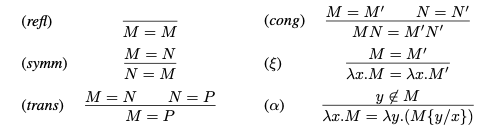
\includegraphics[scale=.6]{images/alpha-equiv}
\end{center}

\alert{Convenția Barendregt:} \\ variabilele legate sunt redenumite pentru a fi distincte.
\end{frame}


%------------------------------------------------

\begin{frame}[fragile]{Substituții}

%Am vorbit despre înlocuirea variabilelor cu variabile (redenumire).

\intens{Vrem să substituim variabile cu lambda termeni.}

\smallskip
\intens{$\subt{M}{N}{x}$} este rezultatul obținut după înlocuirea lui $x$ cu $N$ în $M$.

\smallskip
Trebuie să fim atenți la următoarele cazuri:

\alert{1. Vrem să înlocuim doar variabile libere.} \\
Numele variabilelor legate este considerat imaterial, și nu ar trebui să afecteze rezultatul substituției. \\
De exemplu, \intens{$\subt{\app{x}{(\abs{xy}{x})}}{N}{x}$} ar trebui să fie \intens{$\app{N}{(\abs{xy}{x})}$}, \\ nu {\color{red} $\app{N}{(\abs{xy}{N})}$} sau  {\color{red} $\app{N}{(\abs{Ny}{N})}$}.

\end{frame}

%------------------------------------------------

\begin{frame}[fragile]{Substituții}

\alert{2. Nu vrem să legăm variabile libere neintenționat.} 

De exemplu, fie \intens{$M \equiv \abs{x}{\app{y}{x}}$} și \intens{$N \equiv \abs{z}{\app{x}{z}}$}.

Variabila $x$ este legată în $M$ și  liberă în $N$. 

Ce ar trebui să obținem dacă am substitui $y$ cu $N$ în $M$? \\ Naiv, ne-am gândi la

\vspace{-.2cm}
\begin{center}
\intens{$\subt{M}{N}{y} = \subt{(\abs{x}{\app{y}{x}})}{N}{y} = \abs{x}{\app{N}{x}} = \abs{x}{\app{(\abs{z}{\app{x}{z}})}{x}}$}.
\end{center}

\vspace{-.2cm}
Totuși, nu este ceea ce am vrea să obținem, deoarece $x$ este liber în $N$, iar în timpul "substituției" a devenit legată.

Trebuie să luăm în calcul că $x$-ul legat din $M$ nu este  $x$-ul liber din $N$, \\
și de aceea \alert{redenumim variabilele legate} înainte de substituție.

\vspace{-.2cm}
\begin{center}
\intens{$\subt{M}{N}{y} = \subt{(\abs{x'}{\app{y}{x'}})}{N}{y} = \abs{x'}{\app{N}{x'}} = \abs{x'}{\app{(\abs{z}{\app{x}{z}})}{x'}}$}.
\end{center}

\end{frame}

%------------------------------------------------

\begin{frame}[fragile]{Substituții}

\alert{Substituția} aparițiilor libere ale lui $x$ cu $N$ în $M$, notată cu \intens{$\subt{M}{N}{x}$},\\ este definită prin:

\smallskip
\begin{tabular}{lcll}
$\subt{x}{N}{x}$ & $\equiv$ & $N$ \\
$\subt{y}{N}{x}$ & $\equiv$ & y & dacă $x \neq y$ \\
$\subt{(\app{M}{P})}{N}{x}$ & $\equiv$ & $\app{(\subt{M}{N}{x})}{(\subt{P}{N}{x})}$ & \\
$\subt{(\abs{x}{M})}{N}{x}$ & $\equiv$ & $\abs{x}{M}$ & \\
$\subt{(\abs{y}{M})}{N}{x}$ & $\equiv$ & $\abs{y}{(\subt{M}{N}{x}})$ & dacă $x \neq y$ și $y \not\in FV(N)$\\
$\subt{(\abs{y}{M})}{N}{x}$ & $\equiv$ & $\abs{y'}{(\subt{\sub{M}{y'}{y}}{N}{x}})$ & dacă $x \neq y$, $y \in FV(N)$ \\
&&&  și $y'$ variabilă nouă \\
\end{tabular}

\smallskip
Deaorece nu specificăm ce variabilă nouă alegem, \\ spunem că substituția este bine-definită modulo $\alpha$-echivalențe.
\end{frame}

%------------------------------------------------
\begin{frame}[fragile]{Exerciții}

\textbf{\intens{Exercițiu.}} 
Calculați următoarele substituții:
\begin{enumerate}
	\item \alert{$\subt{(\abs{z}{x})}{y}{x}$} \onslide<2->{\hfill {\color{True} Corect: $\abs{z}{y}$}}

	\smallskip
	\item \alert{$\subt{(\abs{y}{x})}{y}{x}$} 
	\onslide<3->{\hfill {\color{True} Corect: $\abs{y'}{y}$},  {\color{False} Greșit: $\abs{y}{y}$}}

	\smallskip	
	\item \alert{$\subt{(\abs{y}{x})}{(\abs{z}{\app{z}{w}})}{x}$} 
	\onslide<4->{\hfill {\color{True} Corect: $\abs{yz}{zw}$}}	

\end{enumerate}

\end{frame}


%------------------------------------------------
\begin{frame}
  \vfill
  \centering

\textbf{\large \alert{Quiz time!}}


\includegraphics[scale=.35]{../Quiz/C02-Q1.png}

 \url{https://tinyurl.com/C02-Quiz1}
  \vfill
\end{frame}

%%------------------------------------------------
%\begin{frame}[fragile]{$\beta$-reducții}
%
%\alert{Convenție.} Spunem că doi termeni sunt egali, notat \intens{$M = N$},\\ dacă sunt $\alpha$-echivalenți.
%
%\begin{itemize}
%	\item \alert{$\beta$-reducție} = procesul de a evalua lambda termeni prin "pasarea de argumente funcțiilor"
%
%	\item \alert{$\beta$-redex} = un termen de forma \intens{$\app{(\abs{x}{M})}{N}$}
%
%	\item \alert{redusul} unui redex \intens{$\app{(\abs{x}{M})}{N}$} este \intens{$\subt{M}{N}{x}$}
%	
%	\item reducem lambda termeni prin găsirea unui subtermen care este redex, și apoi înlocuirea acelui redex cu redusul său
%	
%	\item repetăm acest proces de câte ori putem, până nu mai sunt redex-uri
%	
%	\item \alert{formă normală} = un lambda termen fără redex-uri
%\end{itemize}
%\end{frame}
%
%%------------------------------------------------
%\begin{frame}[fragile]{$\beta$-reducții}
%
%Un pas de $\beta$-reducție \intens{$\rightarrow_\beta$}  este cea mai mică relație pe lambda termeni care satisface regulile:
%
%\begin{center}
%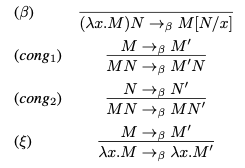
\includegraphics[scale=.6]{images/beta-reduct}
%\end{center}
%
%\end{frame}
%
%%------------------------------------------------
%\begin{frame}[fragile]{$\beta$-reducții}
%
%La fiecare pas, subliniem redexul ales în procesul de $\beta$-reducție.
%
%\begin{center}
%\begin{tabular}{rcl}
%$\app{(\abs{x}{y})}{(\underline{\app{(\abs{z}{\app{zz}})}{(\abs{w}{w})}})}$ & $\rightarrow_\beta$ & $\app{(\abs{x}{y})}{( \subt{(\app{z}{z})}{\abs{w}{w}}{z} )}$ \\ 
%& $\equiv$ & $\app{(\abs{x}{y})}{( \app{(\subt{z}{\abs{w}{w}}{z})}{(\subt{z}{\abs{w}{w}}{z} )}}$ \\
%& $\equiv$ & $\app{(\abs{x}{y})}{(\underline{\app{(\abs{w}{w})}{(\abs{w}{w})}})}$ \\
%& $\rightarrow_\beta$ & $\underline{\app{(\abs{x}{y})}{(\abs{w}{w})}}$ \\
%& $\rightarrow_\beta$ & $y$ \\
%\end{tabular}
%\end{center}
%
%Ultimul termen nu mai are redex-uri, deci este în formă normală.
%
%\end{frame}
%
%%------------------------------------------------
%\begin{frame}[fragile]{$\beta$-reducții}
%
%\begin{center}
%\begin{tabular}{rcl}
%$\app{(\abs{x}{y})}{(\underline{\app{(\abs{z}{\app{zz}})}{(\abs{w}{w})}})}$ & $\rightarrow_\beta$ &  $\app{(\abs{x}{y})}{(\underline{\app{(\abs{w}{w})}{(\abs{w}{w})}})}$ \\
%& $\rightarrow_\beta$ & $\underline{\app{(\abs{x}{y})}{(\abs{w}{w})}}$ \\
%& $\rightarrow_\beta$ & $y$ \\
%\end{tabular}
%\end{center}
%
%\begin{center}
%\begin{tabular}{rcl}
%$\underline{\app{(\abs{x}{y})}{(\app{(\abs{z}{\app{zz}})}{(\abs{w}{w})})}}$ & $\rightarrow_\beta$ & $\subt{y}{\app{(\abs{z}{\app{zz}})}{(\abs{w}{w})}}{x}$ \\ 
%& $\equiv$ & $y$ \\
%\end{tabular}
%\end{center}
%
%Observăm următoarele:
%\begin{itemize}
%	\item reducerea unui redex poate crea noi redex-uri
%	\item reducerea unui redex poate șterge alte redex-uri
%	\item numărul de pași necesari până a atinge o formă normală poate varia, în funcție de ordinea în care sunt reduse redex-urile
%	\item rezultatul final pare că nu a depins de alegerea redex-urilor 
%\end{itemize}
%
%\end{frame}
%
%
%%------------------------------------------------
%\begin{frame}[fragile]{Confluența $\beta$-reducției}
%
%Notăm cu \intens{$M \twoheadrightarrow_\beta M'$} faptul că $M$ poate fi $\beta$-redus până la $M'$ în mai mulți pași  (închiderea reflexivă și tranzitivă a relației $\rightarrow_\beta$).
%
%\bigskip
%\alert{Teorema Church-Rosser.}
%Dac\u a $M \twoheadrightarrow_\beta M_1$ și $M \twoheadrightarrow_\beta M_2$ atunci exist\u a $M'$ astfel încât $M_1 \twoheadrightarrow_\beta M'$ și $M_2\twoheadrightarrow_\beta M'$.
%
%\vspace{-.4cm}
%\begin{figure}[h]
%  \centering
%  \begin{tikzpicture}	
%  	\node(t) at (0,2) {$M$}; 
%	\node(t1) at (-2,1) {$M_1$};
%   	\node(t2) at (2,1) {$M_2$};
%	\node (u) at (0,0) {$M'$};
%	\draw [->>]  (t) -- (t1) ;
%	\draw [->>]  (t) -- (t2) ;
%	\draw [->>, dashed]  (t1) -- (u) ;
%	\draw [->>, dashed]  (t2) -- (u) ;
%   \end{tikzpicture}
%\end{figure} 
%
%\alert{Consecință.} Un lambda termen poate avea cel mult o $\beta$-formă normală, modulo $\alpha$-echivalență.
%\end{frame}
%
%%------------------------------------------------
%\begin{frame}[fragile]{$\beta$-formă normală}
%
%Totuși, există lambda termeni care nu pot fi reduși la o $\beta$-formă normală (evaluarea nu se termină).
%
%\begin{center}
%\begin{tabular}{rcl}
%$\underline{\app{(\abs{x}{\app{x}{x}})}{(\abs{x}{\app{x}{x}})}}$ & $\rightarrow_\beta$ & $\app{(\abs{x}{\app{x}{x}})}{(\abs{x}{\app{x}{x}})}$ \\
%& $\rightarrow_\beta$ & $\ldots$ \\
%\end{tabular}
%\end{center}
%
%Observați că lungimea unui termen nu trebuie să scadă în procesul de $\beta$-reducție; poate crește sau rămâne neschimbat.
%\end{frame}
%
%%------------------------------------------------
%\begin{frame}[fragile]{Exerciții}
%
%\textbf{\intens{Exercițiu.}} 
%Verificați dacă termenii de mai jos pot fi aduși la o $\beta$-formă normală:
%\begin{enumerate}
%	\item \alert{$\app{(\abs{x}{x})}{M}$} \onslide<2->{\hfill {\color{True} Corect: $M$}}
%
%	\smallskip
%	\item \alert{$\app{\app{(\abs{xy}{x})}{M}}{N}$} \onslide<2->{\hfill {\color{True} Corect: $M$}}
%
%	\smallskip
%	\item \alert{$\app{(\abs{x}{\app{x}{x}})}{(\abs{y}{\app{\app{y}{y}}{y}})}$} \onslide<2->{\hfill {\color{True} Corect: $\app{\app{(\abs{y}{\app{\app{y}{y}}{y}})}{(\abs{y}{\app{\app{y}{y}}{y}})}}{(\abs{y}{\app{\app{y}{y}}{y}})}\ldots$}}
%\end{enumerate}
%
%\end{frame}
%
%---------------------------------------------
\begin{frame}
  \vfill
  \centering

\textbf{Pe săptămâna viitoare!}

  \vfill
\end{frame}
\end{document}







